\documentclass[12pt]{extarticle}

\setlength{\headheight}{15pt} % ??? we do what fancyhdr tells us to do  

\title{Mathematical Statistics}
\author{Giacomo Ellero}
\date{a.y. 2024/2025}

\usepackage{preamble}

\newcommand{\cov}{{\operatorfont Cov}}
% Distributions
\newcommand{\Bernoulli}{{\operatorfont Bernoulli}}
\newcommand{\Normal}{{\operatorfont N}}
\newcommand{\GammaD}{{\operatorfont Gamma}}
\newcommand{\Poisson}{{\operatorfont Poisson}}
\newcommand{\Exponential}{{\operatorfont Exponential}}
\newcommand{\BivariateNormal}{{\operatorfont BivariateN}}

\newcommand{\convas}{\xrightarrow{\operatorfont a.s.}}
\newcommand{\convdist}{\xrightarrow{\operatorfont d}}
\newcommand{\convprob}{\xrightarrow{\operatorfont P}}
\newcommand{\convmean}[1]{\xrightarrow{#1}}

\renewcommand{\vec}[1]{\uvec{#1}}

\begin{document}

\firstpage

\section{Descriptive statistics}

\subsection{Introduction}

\begin{definition}{Statistics}{statistics}
    Statistics is the art of modelling situations in which probability plays a role and draw conclusions based on data observed in such situations.
\end{definition}

\textbf{Descriptive statistics} on the other hand will just try to summarize the data in a meaningful way.

\begin{definition}{Statistical model}{statistical-model}
    A statistical model is a collection of probability distributions on a given sample space.
\end{definition}

\begin{example}{Coin toss}
    We have $\Omega = \{ H, T \}$ and assume $P(H) = p$. We have that $X \sim \Bernoulli(p)$. The statistical model of this setup will be
    \begin{equation}
        M = \{ \Bernoulli(p) : p \in [0, 1] \}
    \end{equation}
\end{example}

The meaning of the model is to collect all the possible probability distributions of $X$.

\begin{remark}{Collections of random variables}{}
    Often $X$ is the collection of many observations, hence $X = (X_1, \dots, X_n)$.
    When the $X_i$s are IID we say $X$ is a \textbf{sample}.
\end{remark}

If the $X_i$s are IID we can focus on the marginal $X_i$ and compute $X$ later.

\begin{example}{Sample from population}{}
    Let $N$ be a large number of people composing a population.
    Some proportion $p$ of $N$ has a characteristic $A$.

    We want to estimate $p$ without asking all the $N$ people.

    To do so we choose $n$ people randomly, \textit{without replacement}.
    This type of sampling allows us to assume that $X_i$s are IID.
    Our $X_i$ can be either $1$ (if the person has $A$) or $0$ (if they do not).
    We have that $M$ is a collection of $\Bernoulli$.

    An easy way to estimate $p$ would be
    \begin{equation}
        \hat p = \frac{\# A}{n}
    \end{equation}
\end{example}

We just saw in the example if we sample without replacement $X_i$s are IID.
If we sample \textit{with} replacement we can only approximate IID variables if $N$ is very large.

\begin{example}{Measurement errors}{}
    Assume we have $X_n$ observations and let $c$ be the actual result.
    Let $e_i = X_i - c$ be the error for each measurement.

    We will assume that the experiments are done in the same conditions, independently from the past (giving us IID random variables) and with an expected error equal to $0$.

    In this case $M$ would be the ser of all distributions with expected value $c$ but this is not very useful as it doesn't give us any information.
    A better solution would be to use the $\Normal(c, \sigma^2)$.
\end{example}

\subsection{Validation}

After we created a model we have to do a process called \textbf{model validation} to make sure that we found a good model.
This is because the model we came up with is based on previous observations and we have to verify it still works.

We proceed by repeating the experiment, therefore our random variables become just numbers. We want to measure two properties of these numbers and compare them with the distribution ones:
\begin{itemize}
    \item \textbf{Location}, usually summarized by the \textit{expectation} or the \textit{median};
    \item \textbf{Dispersion}, usually summarized by the \textit{variance} or the \textit{interquartile range}.
\end{itemize}

\begin{remark}{Interquartile range}{}
    The sample interquartile range is the distance between the upper and lower quartiles of the data.
\end{remark}

\begin{definition}{Sample variance}{sample-variance}
    \begin{equation}
        S_X^2 = \frac{1}{n-1} \sum^n_{i = 1}(X_i - \overline X)
    \end{equation}
\end{definition}

Usually if the distribution is \textbf{symmetric} we prefer the \textit{sample mean} and the \textit{variance}; while if the distribution is \textbf{asymmetric} we prefer the \textit{median} and the \textit{interquartile range}.

\subsubsection{Graphical representation of samples}

\begin{figure}[H]
    \centering
    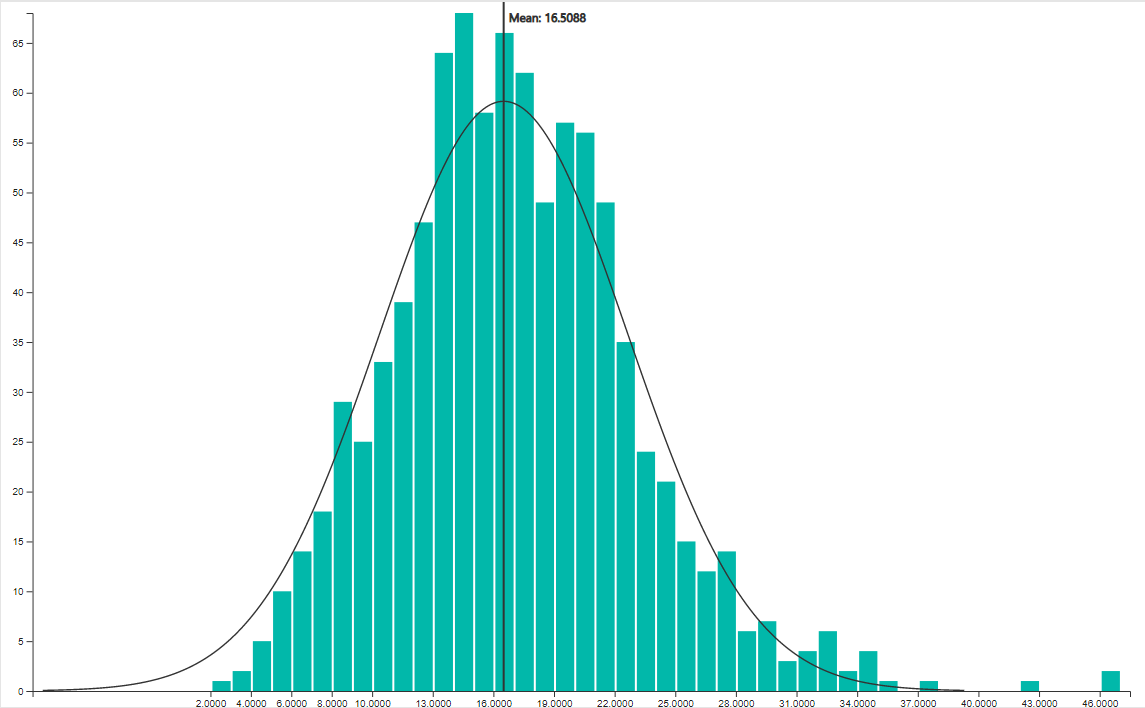
\includegraphics[width=0.75\textwidth]{assets/statistics/histogram.png}
    \caption{A histogram and the graph of the distribution of the samples}
\end{figure}

\begin{figure}[H]
    \centering
    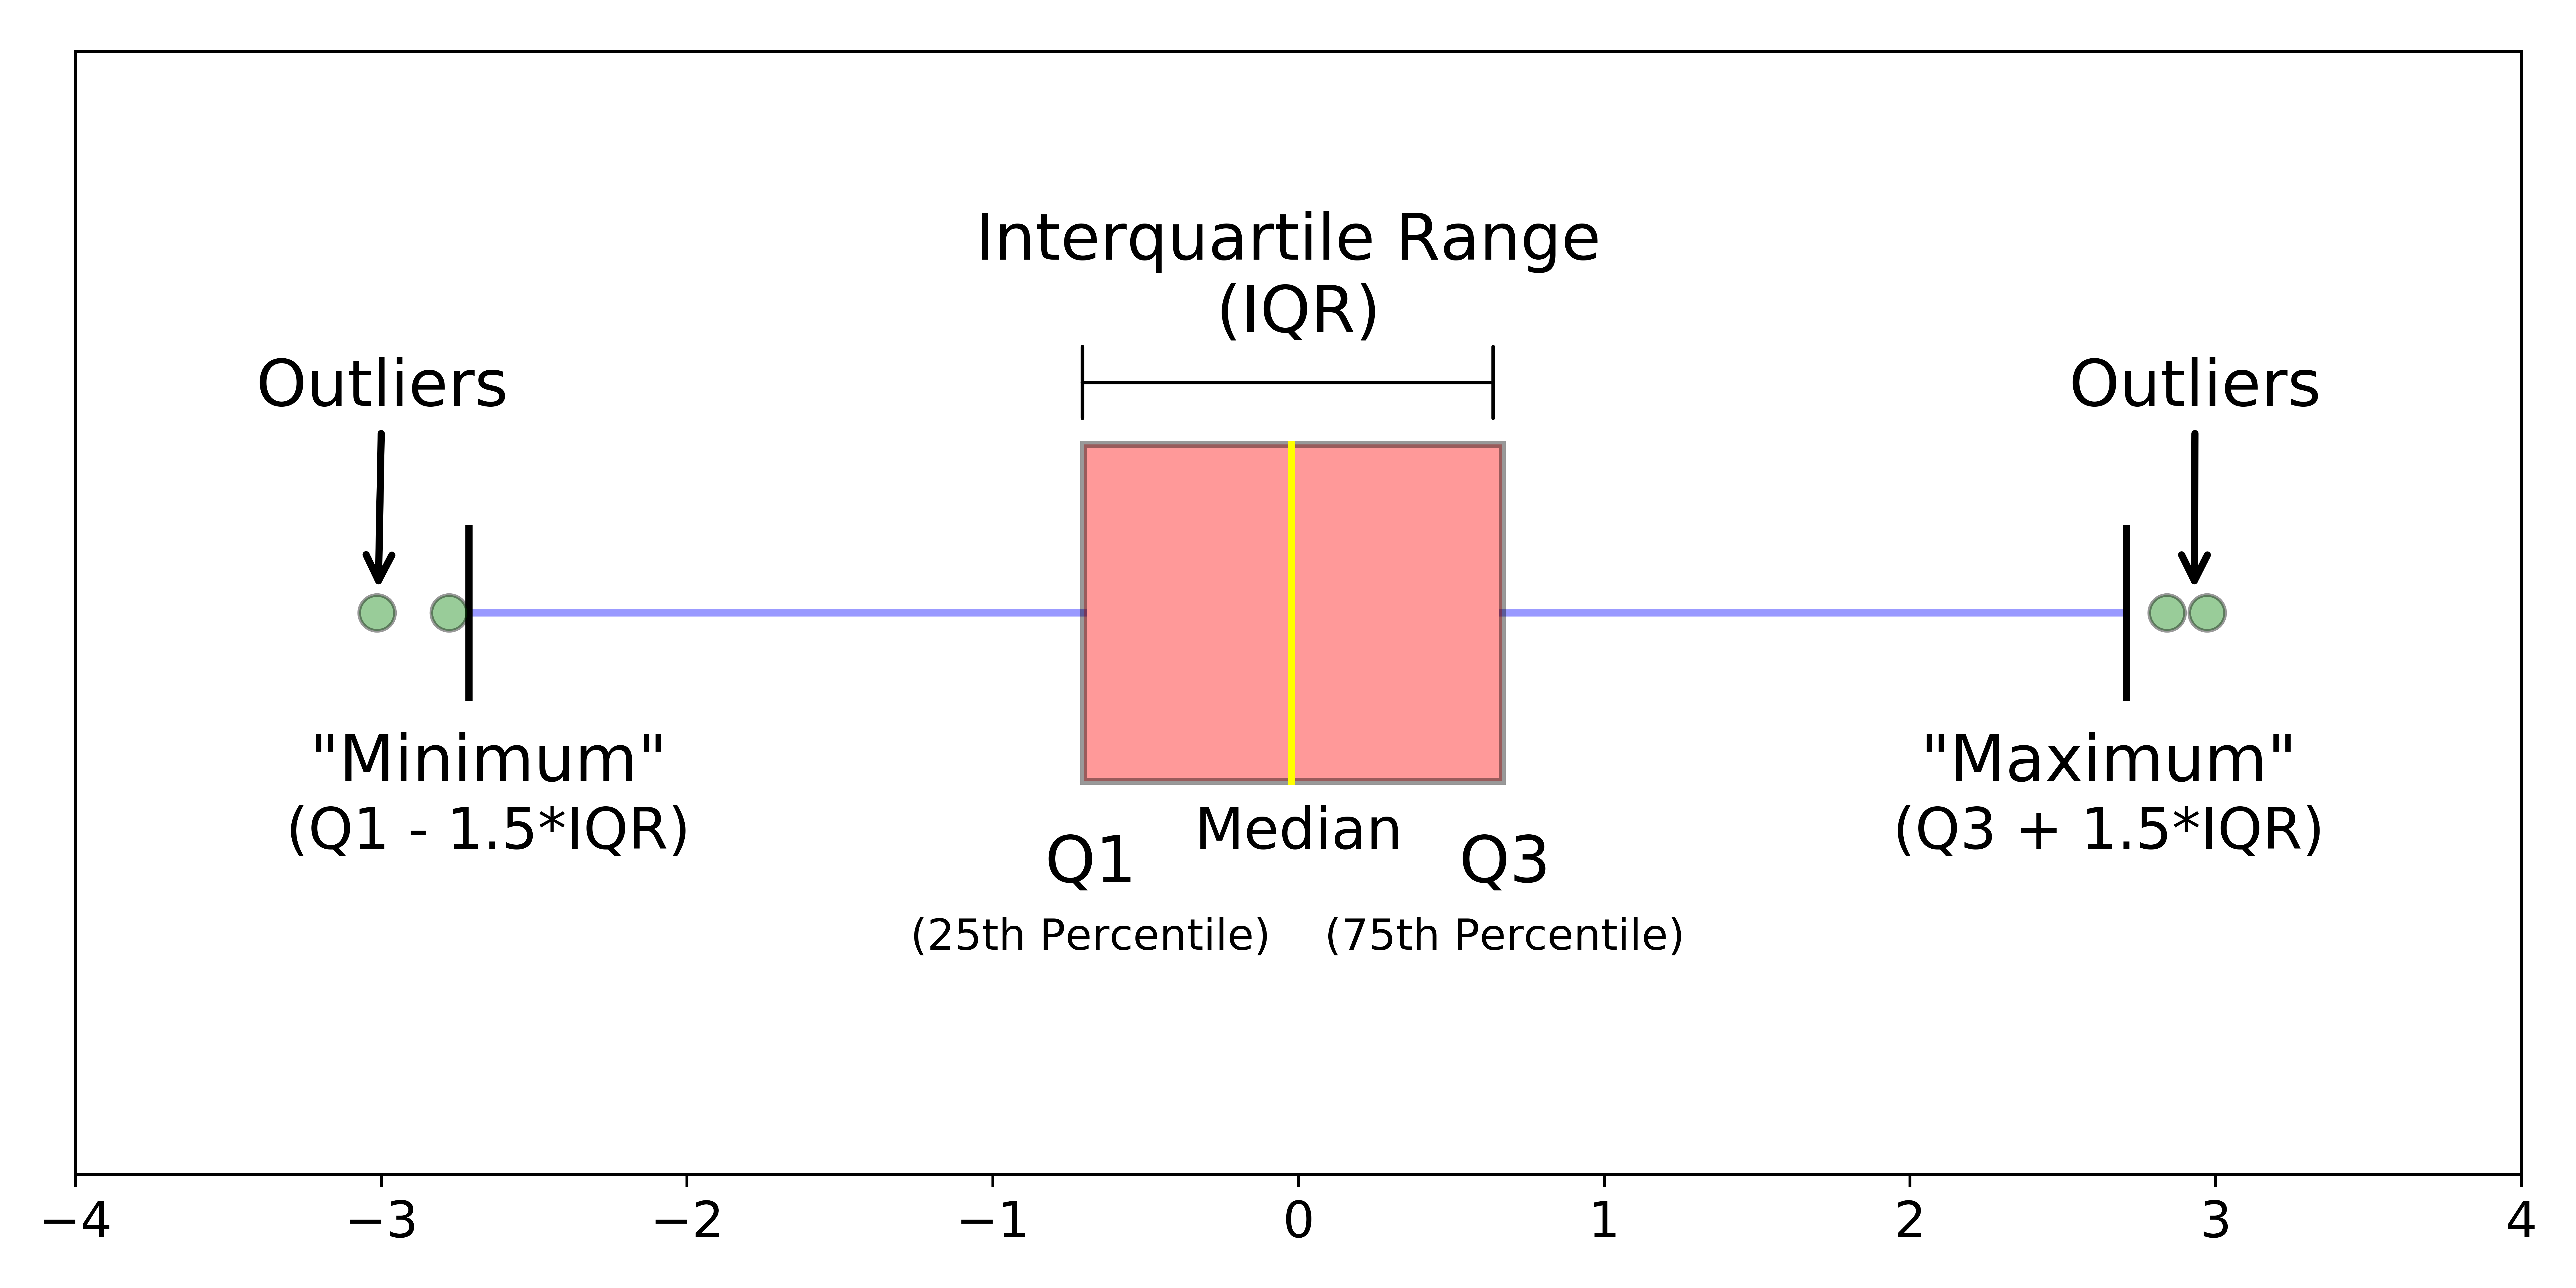
\includegraphics[width=0.75\textwidth]{assets/statistics/boxplot.png}
    \caption{A boxplot with indication on what the lines mean}
\end{figure}

Boxplots are very useful to check the symmetry of a sample.

\subsubsection{Location-Scale family of distributions}

\begin{definition}{Location-Scale family}{location-scale-family}
    Let $X$ be a random variable with distribution $F$ and $Y = a + bX$ with $b>0$.
    Then the distribution of $Y$ is
    \begin{equation}
        F_{a, b}(y) = F\left( \frac{y-a}{b} \right)
    \end{equation}
\end{definition}

\begin{example}{Normal distribution}{}
    $F$ is in the same location-scale family as the standard normal $\iff$ $F$ is a normal distribution
\end{example}

\subsubsection{Quantiles}

\begin{definition}{$\alpha$-quantiles}{alpha-quantiles}
    The $\alpha$-quantile of a distribution $F$ is given by
    \begin{equation}
        F^{-1}(\alpha) = \inf\{ x: F(x) \geq \alpha \}, \quad \alpha \in (0, 1)
    \end{equation}
\end{definition}

The quantile function of a location-scale family is
$F_{a, b}^{-1}(\alpha) = a + bF^{-1}(\alpha)$.

\begin{definition}{QQ-plot}{qq-plot}
    The QQ-plot for the realizations $x_1, \dots, x_n$ for a distribution function $F$ is a plot of the points
    \begin{equation}
        \left\{ \left( F^{-1}\left( \frac{i}{n+1} \right), x_i \right) : i = 1, \dots, n \right\}
    \end{equation}
    where $i$ is the order of the indices of $x_i$ such that they are in \textit{increasing order}.
\end{definition}

If the points $x_1, \dots, x_n$ come from $F$ then the points will approximately align to the $y = x$ line.
This is because we expect the sample quantile $x_i$ to be close to the theoretical quantile given by the formula.

\subsubsection{Correlation and independence}

As we know from Probability, we define the correlation coefficient as
\begin{equation}
    \rho_{A,B} = \frac{\cov(A, B)}{\sigma_A \sigma_B} \in [-1, 1]
\end{equation}

Recall that independence implies $\rho = 0$, but not viceversa (except for the normal distribution).

\begin{definition}{Sample correlation coefficient}{sample-correlation-coeff}
    Consider a sample of pairs $(X_1, Y_1), \dots, (X_n, Y_n)$.
    Then we define the sample correlation coefficient as
    \begin{equation}
        r_{X, Y} = \frac{\sum^n_{i = 1} (X_i - \overline{X})(Y_i - \overline{Y})}{(n-1)\sqrt{S^2_X} \sqrt{S^2_Y}}
    \end{equation}
\end{definition}

In the definition we use the following notation:
\begin{itemize}
    \item $\overline X$ is the sample mean
    \item $\sqrt{S^2_X}$ is the sample variance
\end{itemize}

We observe the following from $r_{X, Y}$:
\begin{itemize}
    \item $r_{X, Y} \in [-1, 1]$.
    \item If $r_{X, Y} = 1$ all the samples lie on the line $y = \overline y + \frac{S_y}{S_x}(x-\overline x)$.
    \item If $r_{X, Y} = -1$ all the samples lie on the line $y = \overline y - \frac{S_y}{S_x}(x-\overline x)$.
    \item If $X_1, \dots, X_n$ and $Y_1, \dots, Y_n$ are independent then $r_{X, Y}$ will be close to $0$.
\end{itemize}

Graphically we can observe correlation or independence using \textbf{scatter plots}: if the graph of $\{ (x_i, x_{i+1}) : i = 1, \dots, n-1 \}$ should show not much of a structure if the samples are independent.

\subsection{Estimation}

Estimation is the process of finding the best fitting distribution from the statistical model.

Suppose the model depends on an unknown parameter $\theta \in \Theta$:
\begin{equation}
    \mathcal M = \{ P_\theta : \theta \in \Theta \}
\end{equation}
Now we assume that $X = (X_1, \dots, X_n)$ has distribution $P_\theta$ for some $\theta \in \Theta$.
Then we want to find the $\theta$ that makes $P_\theta$ best fit the observed data.
We call this the \emph{true value of $\theta$}.
Sometimes it is even useful to compute the true value of some $g(\theta)$.

\begin{definition}{Estimator}{estimator}
    An \emph{estimator} is a random vector $T(X)$ that depends only on the observation $X$.

    The corresponding \emph{estimate} for a realization $x$ is $T(x)$.
\end{definition}

Note that estimators \emph{do not} depend on $\theta$.
The estimate will give us our value of $\theta$.

First, lets define some notation:
\begin{itemize}
    \item $T$ is the estimator $T(X)$.
    \item $t$ is the estimate $T(x)$.
    \item $\hat \theta$ is used for both the estimator and estimate of a unknown $\theta$ of interest
\end{itemize}

We could use as an estimator the distance between $T$ and $g(\theta)$
\begin{equation}
    \norm{T - g(\theta)}
\end{equation}

We want this difference to be as small as possible, that is, to be as concentrated as possible towards $0$.
Since $\norm{T - g(\theta)}$ is a random variable we can consider the one more concentrated around $0$.

\newcommand{\MSE}{{\operatorfont MSE}}

\begin{definition}{Mean squared error}{mean-squared-error}
    The mean squared error MSE of an estimator $T$ for the value of $g(\theta)$ is defined as
    \begin{equation}
        \MSE(\theta, T) = E_\theta\left(\norm{T - g(\theta)}^2\right)
    \end{equation}
    where $E_\theta$ is the expectation of $P_\theta$
\end{definition}

\begin{proposition}{MSE decomposition}{mse-decomposition}
    If a $T$ is real-valued estimator we can decompose the $\MSE$ as
    \begin{equation}
        \MSE(\theta, T) = V_\theta(T) + (E_\theta(T) - g(\theta))^2
    \end{equation}
\end{proposition}
\begin{proof}
    \begin{align}
        E_\theta\left((T - g(\theta))^2\right) & = E_\theta\left((T -E_\theta(T) + E_\theta(T) - g(\theta))^2\right)                                                            \\
                                               & = E_\theta(T-E_\theta(T))^2 - 2E_\theta(T-E_\theta(T))(E_\theta(T) - g(\theta)) + \cancel{E_\theta}(E_\theta(T) - g(\theta))^2 \\
                                               & = V_\theta(T) - 2 (E_\theta(T) - g(\theta)) \cancelto{0}{E_\theta(T-E_\theta(T))} - (E_\theta(T) - g(\theta))^2                \\
                                               & = V_\theta(T) - (E_\theta(T) - g(\theta))^2
    \end{align}
\end{proof}

We say that an estimator is \emph{biased} if it's expectation is not centered around $g(\theta)$.

\begin{definition}{Likelihood function}{likelihood-function}
    Let $X$ be a random vector with pdf $p_0$ that depends on a parameter $\theta \in Theta$.
    For a fixed $x$ the likelihood function is defined as
    \begin{equation}
        \theta \mapsto L(\theta, x) = p_\theta(x)
    \end{equation}
\end{definition}

\begin{lemma}{IID variables}{}
    If $X_1, \dots, X_n$ IID then
    \begin{equation}
        L(\theta; X_1, \dots, X_n) = \prod_{i = 1}^{n} L(\theta, X_i)
    \end{equation}
\end{lemma}

\begin{definition}{Maximum likelihood estimator}
    The maximum likelihood estimate of $\theta$ is the value $T(x) \in \Theta$ that maximizes the likelihood function $L(\theta; x)$.

    The maximum likelihood estimator is $T(X)$.
\end{definition}

An useful trick we can use to find the maximum likelihood estimate is to apply the $\log$ to the likelihood function.
In this way we are left to deal with sums and not products (by the properties of logarithms), and, since $\log$ is monotone, the maximum of the transformation will be the maximum of the original function.

We will call \textbf{score function} the derivative of the likelihood function (or its log transformation).

\end{document}
